
\oursection{Design}
We designed \name{}, a web server for image searching which runs on commodity hardware.
It compares incoming images and Google street view images, results geological location of the street art in the input image.

\oursubsection{Overall Architecture}

\begin{figure}[t]
	\centering
	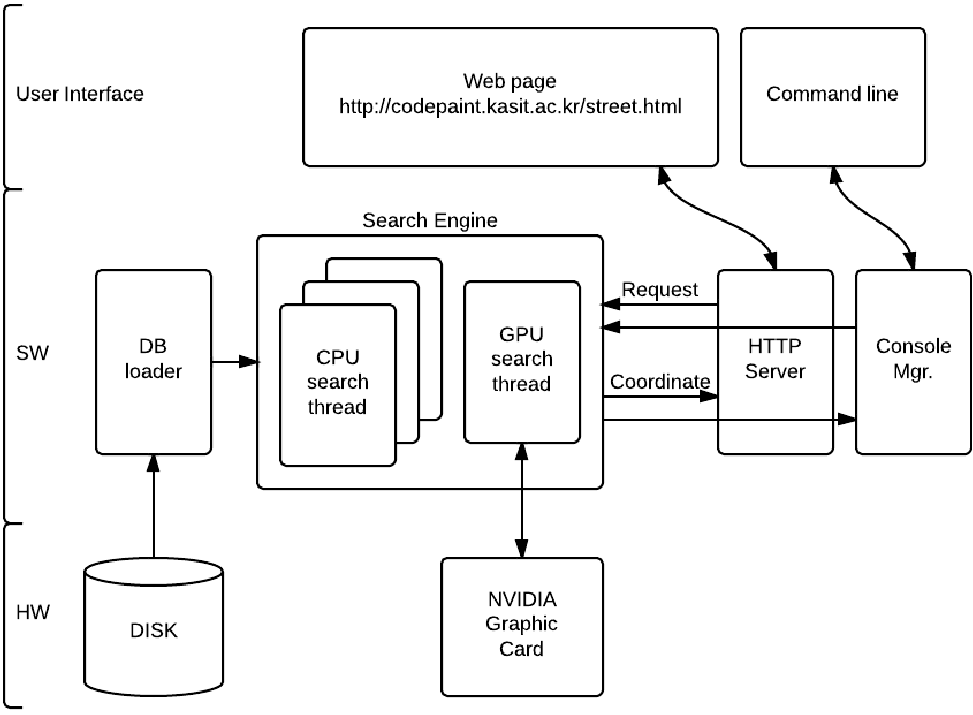
\includegraphics[scale=0.50]{figs/arch}
	\vspace{-0.1in}
	\ourcaption{Overall architecture of \name{}}
	\vspace{-0.1in}
	\label{fig:arch}
\end{figure}

\name{} is composed of DB loader module, search engine module and HTTP server module.
When the image search request arrives via HTTP server module, search engine module does vector matching between the input and database loaded by DB loader module.
The database, DB, which is consists of many pairs of geo-location and feature vector is generated before running the \name{} by applying SURF to street view images.
The search engine module use both CPU and GPU resource to minimize the searching time cost.
After the searching is finished, it notice the most probable geological location to the HTTP server module.
Then HTTP server generates HTML code and respond the request.

\oursubsection{DB Loader}
DB loader hides latency of reading DB file by dividing the DB into chunks and prefetching the next chunk to be used while the search engine is processing current chunk.
It has a large size, typically several GB, of ring buffer to read DB.
%It has a ring buffer and a large size of memory cache.


%\textbf{Cache eviction policy:}
%\note{TBD}

\oursubsection{Search Engine}
Search engine is a key component of \name{}.
When other modules such as HTTP server request searching to the search engnine, the request does not processed immediately.
Instead, it is enqueue the request to a queue in the search engine and process them by FIFO order.
After searching, the search engine replies the request with only one geological location and its score which indicates how reliable the result is.

It maintains worker thread pool and distributes the searching job to them.
There is two types worker threads, one uses CPU and the other uses GPU.
Usually a search engine have CPU worker threads as many as the number of the machine's logical cores and GPU worker threads as many as the number of general purpose graphic cards.
Each worker thread requests a part of DB to the DB loader and process it repeatedly until the entire DB is processed.
After then, the result from each worker thread is merged by one of the worker thread.

\oursubsubsection{Score of Geological Locations}
Image searching with SURF results many geo-location candidates for a single input image.
We assume that the candidate which has many well-matched vectors is the most probable candidate.
SURF calculates ratio of best-fit distance and second-fit distance for each vector matching.
The best-fit distance is a minimum eucladian distance between a vector of needle and one of vectors of haystack.
The second-fit distance is the secondary minimum in same mannar.
If the ratio is higher than certain level, on the other words, best-fit distance is not very different from second-fit distance, original SURF discards the matching.
We do not discard matching even though the ratio described above is poor, however, we calculate score for each vector matching,
$u = 1 - (best\_fit\ distance / second\_fit\ distance)$.
$u$ means the uniqueness of the matching.
Score of geo-location candidates which have zero or more matched vectors is sum of $u$ of each vector matching.
The search engine selects a candidate with the highest score as a geo-location for the input image.

\oursubsubsection{Parallel Processing}

%\begin{figure}[!t]
%	\begin{separation}
%		\textbf{\em Merging} 
%		\vspace{-0.4cm}
%		\separator
%		\vspace{-0.2cm}
%		For two different search results from two different part of DB
%		\smallskip
%		\begin{compactitem}
%		\item[\bf Input:] $r_A$ and $r_B$
%		\item[\bf Output:] $r_M$
%		\end{compactitem}
%		\medskip
%		\begin{compactenum}[\sl 1.]
%		\item {\bf if } $r_A.best\_dist \le r_B.best\_dist$
%		\item \note{TBD}
%		\end{compactenum}
%
%		\vspace{-0.2cm}
%	\end{separation}
%	\caption{Algorithm description of merging}
%	\label{fig:merging}
%\end{figure}

SURF's vector matching algorithm is highly parallelizable since there is no data dependency between each vector matching.
The DB is usually splitted into many small pieces before searching and the splitted search result is merged into single one after the searching.
Result of each splitted piece of DB is in an intermediate form to be merged with results from other pieces.
Hence our scoring algorithm requires second-fit distance of each vector matching so the intermediate result is consists of geo-location of best-fit vector, best-fit distance and second-fit distance.
The merged result have new best-fit distance and second-fit distance among all unmerged results.
A score of vector matching is computed after all the merging is finished.

\oursubsubsection{GPU Worker}
Nvidia provides General Purpose GPU, GPGPU, and its programming environment, CUDA.
GPU is parallel computing resource separated from CPU.
We can boost up searching process by offloading some part of computation to GPU.
However, copying DB from memory to GPU via PCI bus involves long delay so GPU worker thread should minimize the overheady by requesting large enough portion of DB to DB loader.
%Caching the DB in graphic card memory can be helpful to avoid memory copy between main memory and graphic card memory.

\oursubsection{HTTP Server}
HTTP server module provides web interface to users over the internet.
It handles client's page request, search request and its attatched images.
It converts input images to a set of vectors by doing SURF and deliver it to the search engine module.
After searching, it serves result web page to the client.

\textbf{Handling burst or unfinished requests:}
Even though very optimized implementation of the search engine, image searching is still quite a long job.
Pending burst search request with image file may drain memory resource.
To avoid memory drain and guarantee quality of the service, we only holds limited number of request.
The HTTP server has limited number, 10 for current implementation, of pre-allocated request buffer.
Each buffer has timer that records when the request arrived to handle unfinished request.
When a new request arrives and no buffer is available, it find the oldest request buffer and evict it if it is older than 1 minutes.
Currently, timeout is not implemented.
